\section{Movimiento Rectilíneo Uniforme}

Podríamos decir que uno de los objetivos principales de la mecánica es poder realizar predicciones sobre el movimiento de una partícula, conocido su estado inicial de movimiento.

Ahora bien, de acuerdo con lo estudiado en la sección anterior, uno podría imaginar que la velocidad instantánea de una partícula varía de cualquier forma a medida que transcurre el tiempo. De esta manera, realizar predicciones del comportamiento de la partícula, se volvería una tarea súmamente complicada. En vistas de ello, nos restringiremos en este capítulo a los movimientos más simples: el Movimiento Rectilíneo Uniforme y el Uniformemente Variado. Comenzaremos por el primero y, luego de aprender el concepto de aceleración, veremos el segundo tipo de movimiento.

Uno podría pensar que se está perdiendo de mucha información si se limita a estudiar el movimiento rectilíneo. Pues bien, en los próximos capítulos veremos que, en muchas situaciones cotidianas, basta con estos dos tipos de movimiento para describir el comportamiento de los cuerpos, y que combinando estos dos se pueden describir movimientos más complejos como el tiro parabólico.

El {\bf Movimiento Rectilíneo Uniforme (MRU) es un movimiento con rapidez constante en una trayectoria rectilínea}. Decir que la trayectoria es rectilínea significa decir que el vector velocidad instantánea se mantiene sobre una recta determinada. Que el movimiento sea uniforme implica que la rapidez es constante. Que la rapidez sea constante significa que el módulo de la velocidad permanece invariable a lo largo del tiempo. Dado que no existe en la naturaleza ningún cuerpo capaz de cambiar el sentido de su vector velocidad sin antes detenerse\footnote{Más adelante estudiaremos el caso de partículas que cambian el sentido de su movimiento muy rápidamente y veremos que siempre existe un pequeño intervalo de tiempo, muy corto para que nosotros lo percibamos, en el que la partícula cambia el sentido de su movimiento.}, esto también significa que la velocidad siempre apuntará en el mismo sentido. Como, al mismo tiempo, la dirección, el módulo y el sentido del vector velocidad permanecen constantes, podemos decir que la velocidad instantánea es un vector constante. Lo expuesto hasta aquí se puede resumir en un mapa conceptual:

\begin{figure}[!h]
  \centering
  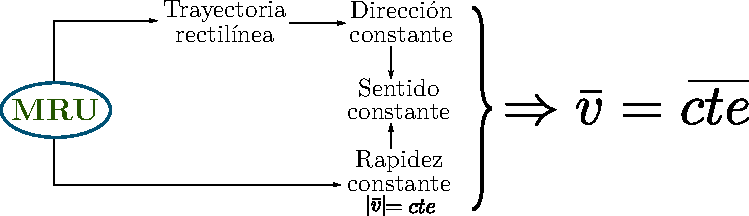
\includegraphics[scale=1]{img/cuadro_MRU.pdf}
\end{figure}

Dado que la velocidad es constante, en todo momento esta será igual a la velocidad media, por lo que
$$\mathbold{\bar{v}}=\mathbold{\bar{v}_m}=\frac{\mathbold{\Delta \bar{x}}}{\Delta t}$$
De esta manera, también se cumple que $\mathbold{\bar{v}} \Delta t=\mathbold{\Delta\bar{x}}$.

Dado que solo tenemos una dimensión, podemos hacer los cálculos directamente utilizando las componentes de los vectores involucrados. Así, podemos escribir:
$${v}(t-t_0)={x}-{x}_0$$
Si despejamos ${x}$ en la ecuación anterior obtenemos
$${x}={x}_0+{v}(t-t_0)$$
o bien
\begin{center}
{\color{NavyBlue}  \boxed{\mathbold{{x}={x}_0+{v}\Delta t}}}
\end{center}

La ecuación anterior se conoce como {\em ``Ley de movimiento del MRU''} o {\em ``Ley horaria''}, y nos permite determinar la posición de una partícula en cada instante de tiempo, conocida su velocidad y su posición inicial.

En muchas situaciones de interés, esta ecuación se puede simplificar tomando $t_0=0$, y así nos queda $${x}={x}_0+{v}t$$
Vamos a ver cómo se utiliza la ley de movimiento en una situación práctica:

\begin{example}{Ejemplo:}
  {\it Un juego muy popular antes del advenimiento de Internet era ``la bolita''. Un tiempo después de haber sido disparada, una bolita de vidrio se encuentra a 20 cm de una pared y se mueve con una rapidez constante de 0,5 m/s alejándose de la misma. Determina a qué distancia se encontrará de la pared al cabo de 2 s, 4 s, 6 s, y 8 s.}
  \tcblower
  {\sf {\bf Modelo:} Supondremos en este problema que la bolita es una partícula que se mueve en una trayectoria rectilínea con rapidez constante.}
  
El primer paso para resolver un problema de física es realizar un esquema de la situación física identificando los datos del problema:
  \begin{center}
    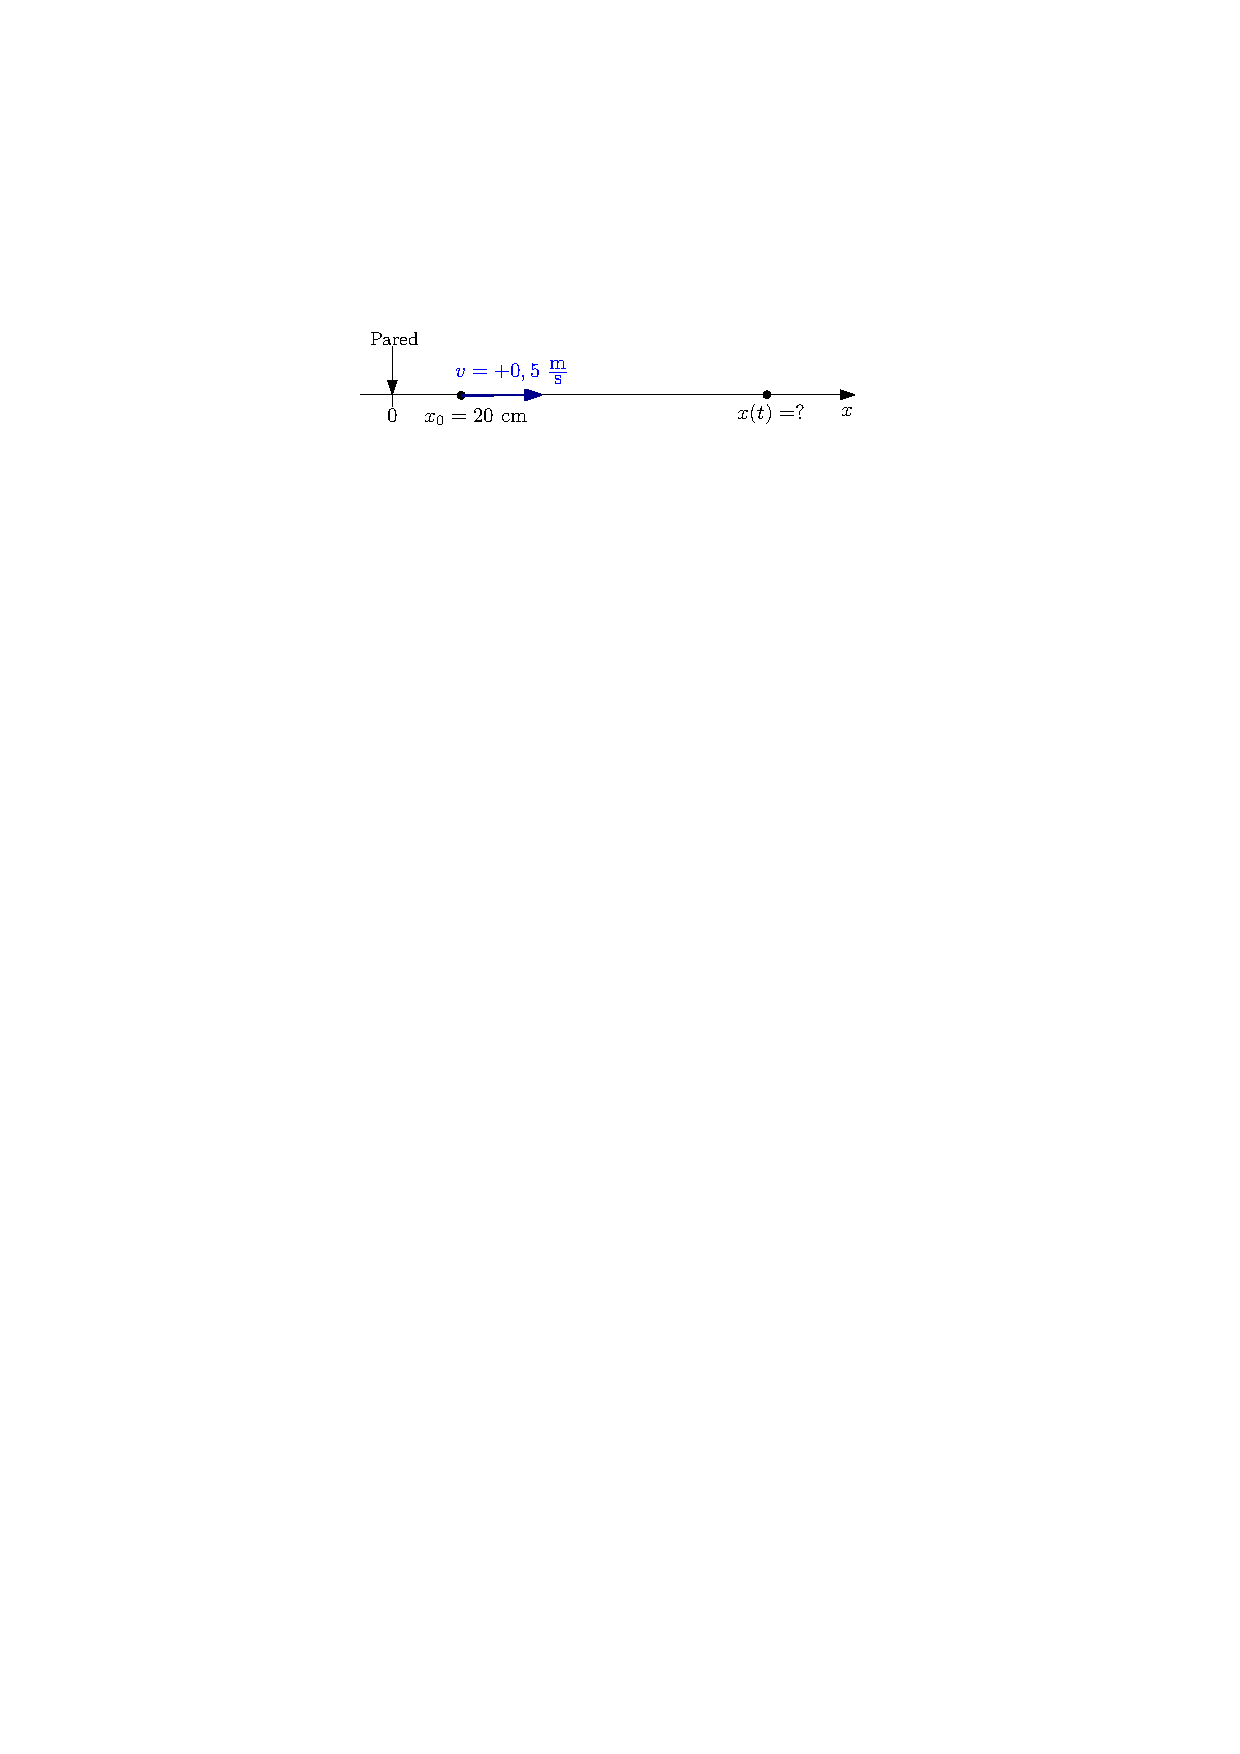
\includegraphics[]{img/bolita.pdf}
  \end{center}
  Dado que hemos colocado el origen de coordenadas de nuestro sistema de referencia en la pared, determinar la distancia de la bolita a la pared significa determinar la posición de la bolita en {\em nuestro} sistema de referencia.
  Debemos procurar que todos los datos estén en el mismo sistema de unidades. En nuestro caso, la posición inicial de la bolita está en un submúltiplo del metro, así que la expresamos en metros: $x_0=0.20$~m. Tomaremos para este problema, $t_0=0\si{s}$.

  Ahora que ya tenemos todos los datos, podemos utilizarlos para calcular la posición de la bolita respecto de la pared en los instantes pedidos:
  $$2\si{s}:\quad x = x_0 + vt = 0.20\si{m} + 0,5\sif{m}{s} \cdot 2\si{s} = 1.20\si{m}$$
  $$4\si{s}:\quad x = x_0 + vt = 0.20\si{m} + 0,5\sif{m}{s} \cdot 4\si{s} = 2.20\si{m}$$
  $$6\si{s}:\quad x = x_0 + vt = 0.20\si{m} + 0,5\sif{m}{s} \cdot 6\si{s} = 3.20\si{m}$$
  $$8\si{s}:\quad x = x_0 + vt = 0.20\si{m} + 0,5\sif{m}{s} \cdot 8\si{s} = 4.20\si{m}$$
\end{example}

La información del Ejemplo anterior se puede volcar en una gráfica en la que representemos la posición de la bolita a medida que transcurre el tiempo. Para realizar este tipo de gráficas, decimos que {\bf la posición es función del tiempo} y lo notamos $\mathbold{x=x(t)}$. La gráfica en cuestión se muestra en la Figura~\ref{fig:grafica_MRU_x}.


\begin{figure}[!h]
  \centering
  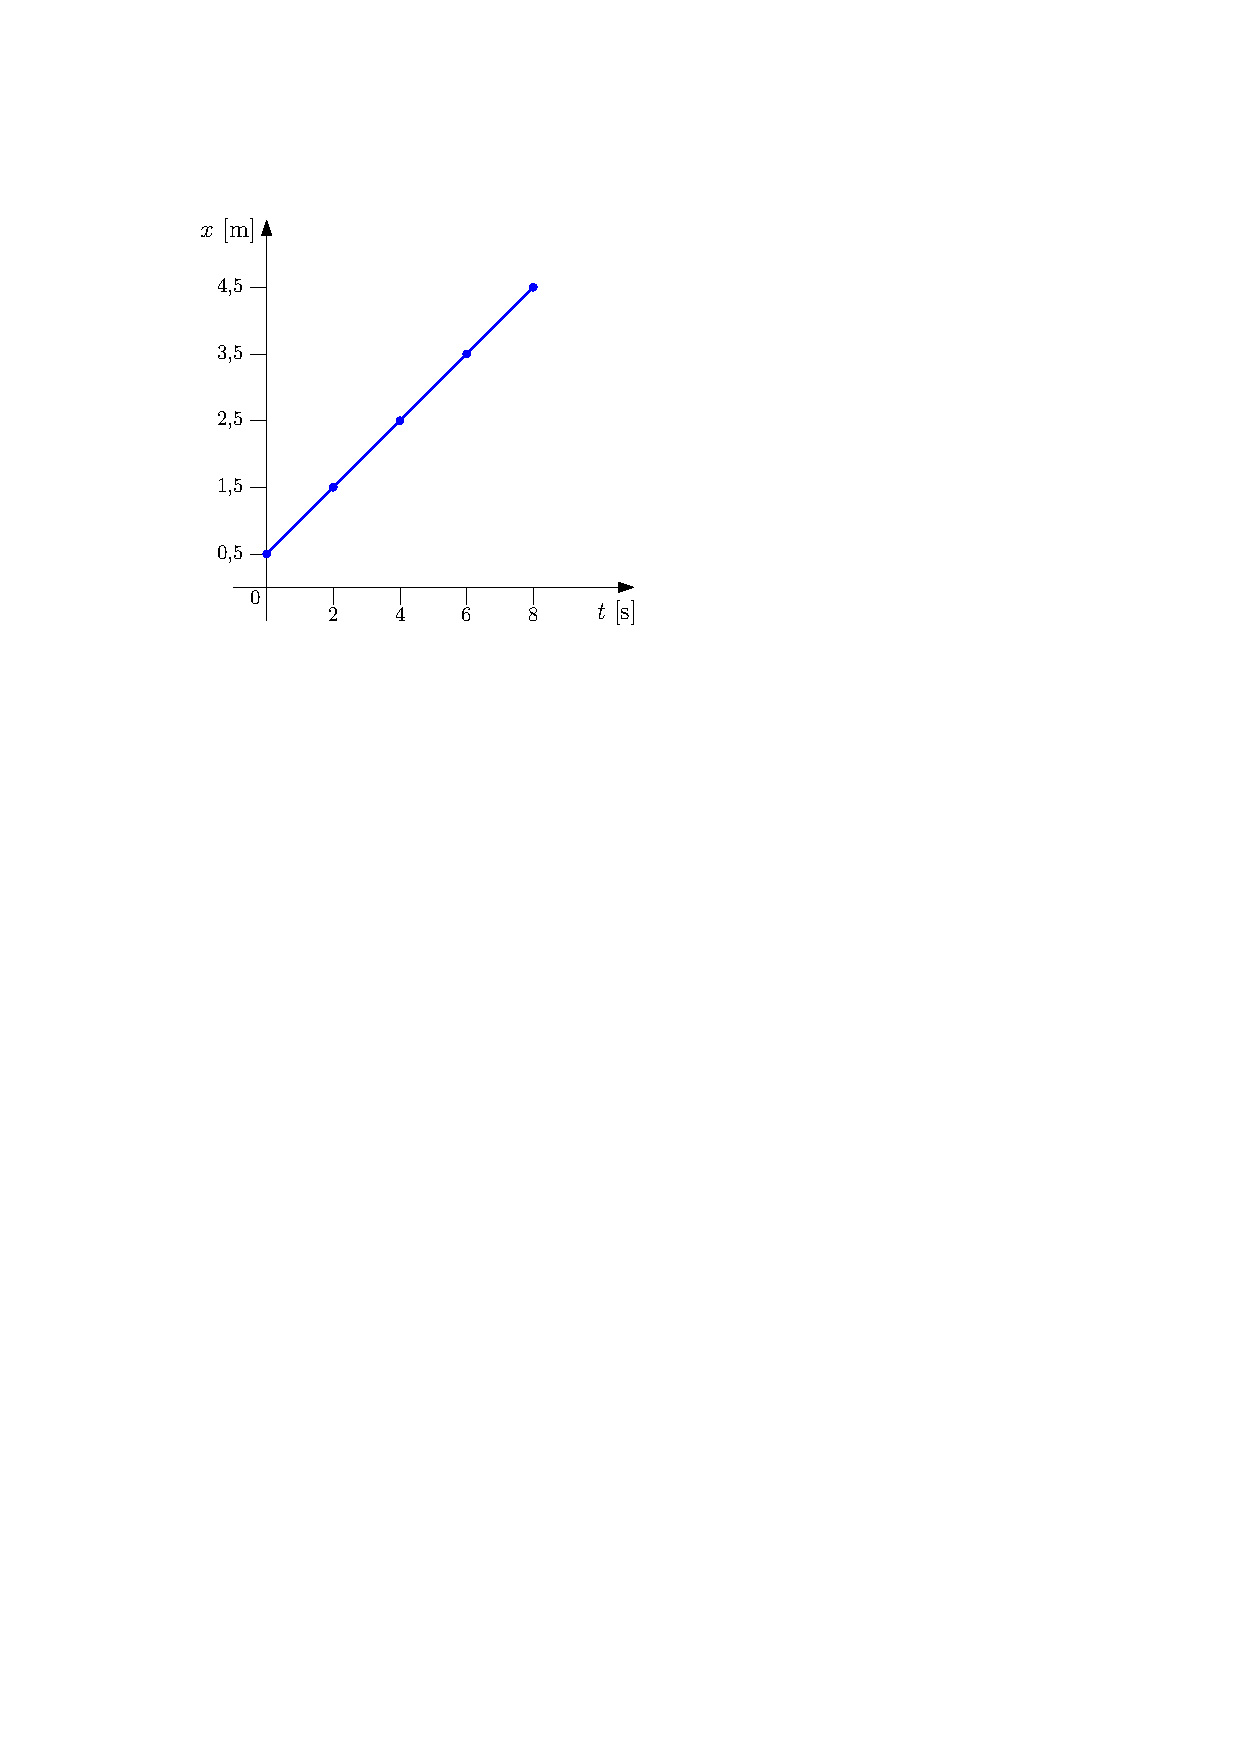
\includegraphics[scale=1]{img/grafica_MRU_x.pdf}
  \caption{\label{fig:grafica_MRU_x} Gráfica típica $x=x(t)$ de un MRU.}
\end{figure}

¿Qué podemos decir de esta gráfica? Lo primero que podemos ver, es que los puntos que se obtienen al graficar están alineados sobre una misma recta. Esto también pasará para cualquier otro instante de tiempo en este mismo movimiento. ¿Por qué? Porque al ser la rapidez constante, {\em en tiempos iguales nuestra bolita recorrerá distancias iguales}. Esta es una de las principales características del Movimiento Rectilíneo Uniforme: La gráfica $x=x(t)$ siempre será una recta.

Otra cosa que observamos de la gráfica, es que la recta corta al eje de las ordenadas en un valor que es ni más ni menos que la posición inicial $x_0$ de la partícula.

También vemos que, a medida que transcurre el tiempo, la posición va tomando valores positivos cada vez mayores. Esto es consistente con el enunciado del problema y con el sistema de referencia elegido: {\em A medida que transcurre el tiempo, la bolita se va alejando del origen de coordenadas, situado en la pared, en el sentido elegido como positivo para el sistema de referencia.}

Grafiquemos ahora la velocidad de nuestra partícula a medida que trancurre el tiempo. Nuestra tarea ahora es mucho más sencilla, puesto que el módulo y el sentido de la velocidad se mantienen constantes a lo largo del tiempo. La gráfica $v=v(t)$ es, entonces, una recta horizontal, como lo muestra la Figura~\ref{fig:grafica_MRU_v}.

\begin{figure}[!h]
  \centering
  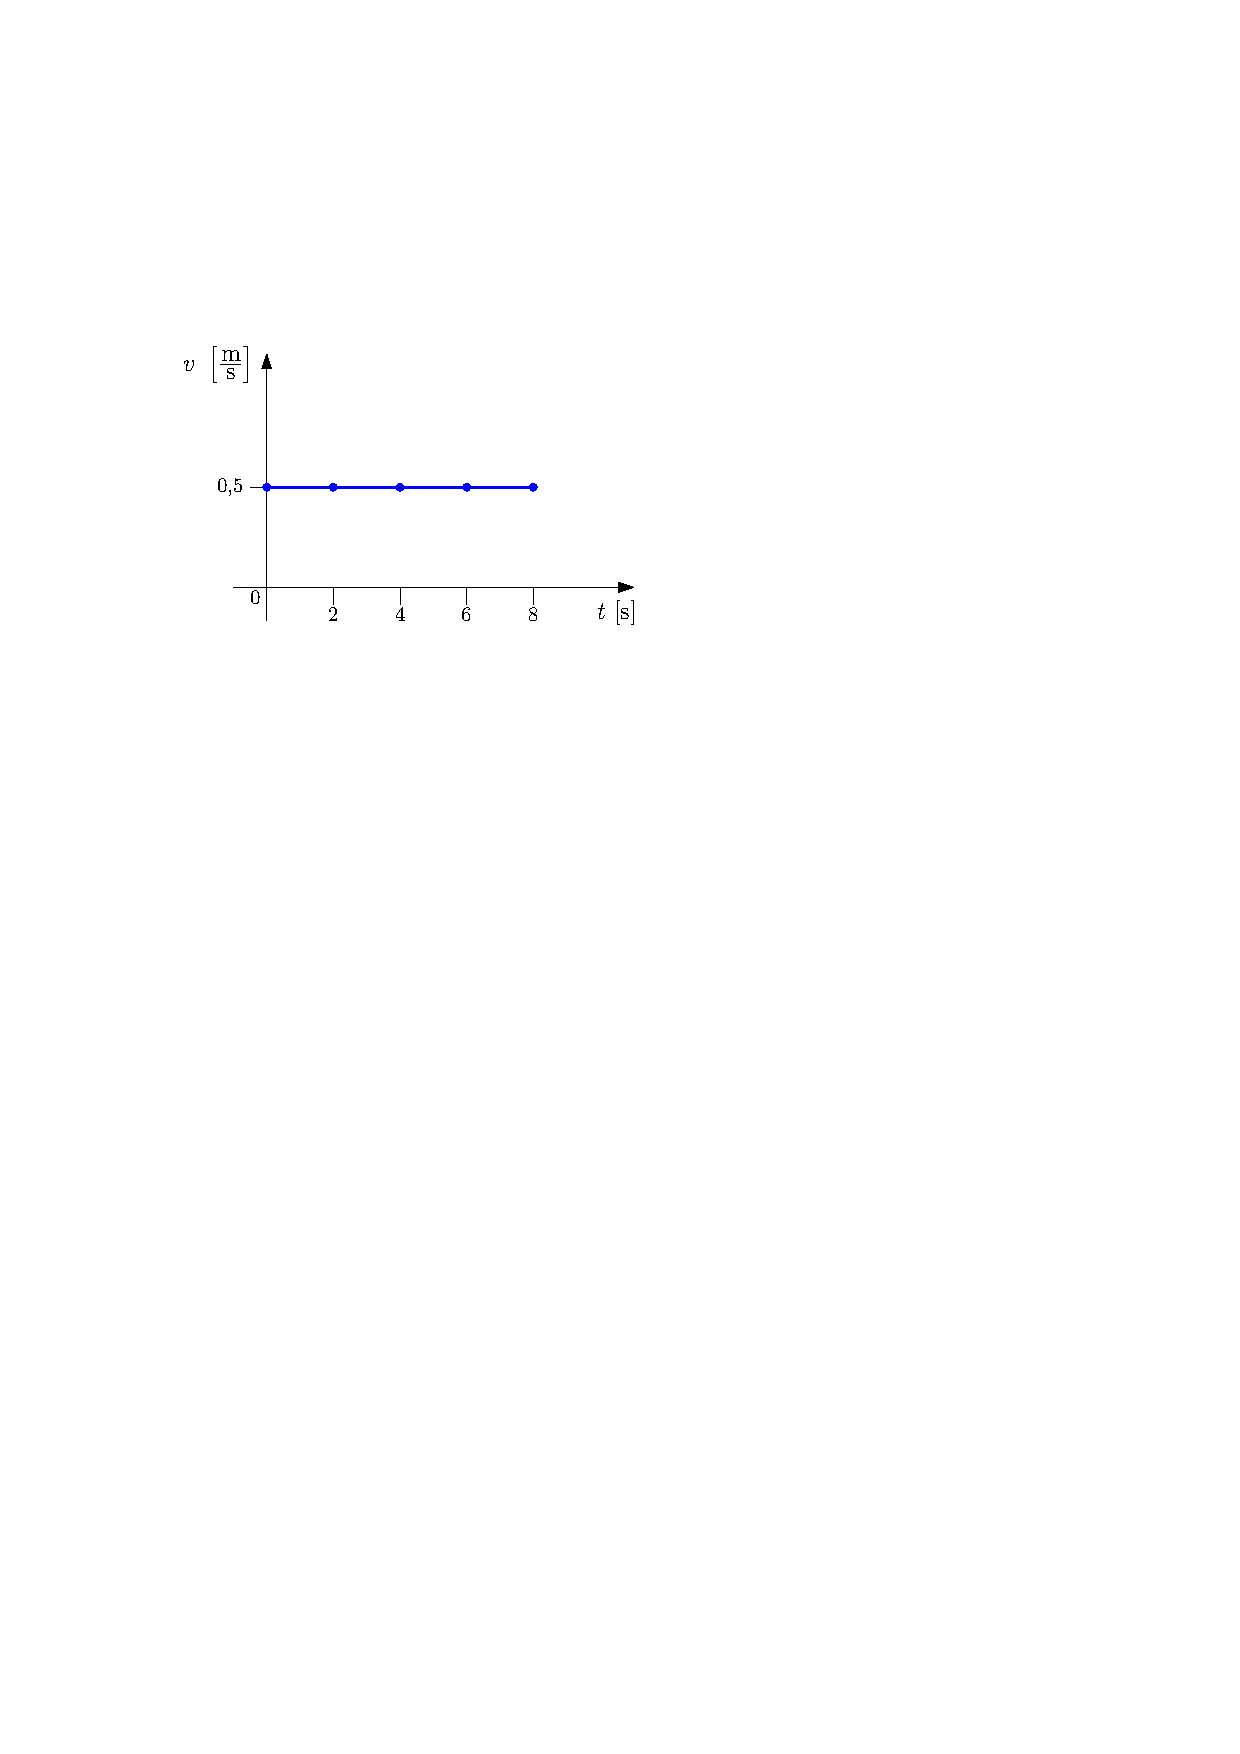
\includegraphics[scale=1]{img/grafica_MRU_v.pdf}
  \caption{\label{fig:grafica_MRU_v} Gráfica típica $v=v(t)$ de un MRU.}
\end{figure}

De esta gráfica podemos decir que la bolita tiene rapidez constante, y que el signo de la velocidad es positivo. Como el signo de la velocidad nos indica el sentido en el que la partícula se está moviendo, podemos decir que nuestra partícula se mueve en el sentido elegido como positivo, lo que es, nuevamente, consistente con el enunciado del problema, con el sistema de referencia que escogimos y, ahora también, con la gráfica $x=x(t)$ que analizamos anteriormente.

\info{Luego de realizar la gráfica de un movimiento cualquiera, uno siempre debe analizarla para corroborar que es consistente con el problema que acaba de resolver. Analizar una gráfica significa extraer de ella toda la información posible. Así, viendo las Figuras~\ref{fig:grafica_MRU_x} y \ref{fig:grafica_MRU_v}, deberíamos poder extraer la siguiente información: {\em Las gráficas muestran un móvil que originalmente se encuentra a $+0.5\si{m}$ del origen de coordenadas y, a medida que transcurre el tiempo, se va alejando del mismo, moviéndose en el sentido elegido como positivo para el sistema de referencia, con rapidez constante.}}

%%%%%%%%%%%%%%%%%%%%%%%%%%%%%%%%%%%%%%%%%%%%%%%
%   Cuadrito que habla sobre la pendiente     %
%%%%%%%%%%%%%%%%%%%%%%%%%%%%%%%%%%%%%%%%%%%%%%%
\begin{mybox}{Para profundizar}
  Si en la gráfica $x=x(t)$ del MRU elegimos un intervalo de tiempo $\Delta t_1$ y buscamos el desplazamiento $\Delta x_1$ que le corresponde, nos queda determinado un triángulo rectángulo $\overset{\triangle}{abc}$. Si ahora elegimos otro intervalo $\Delta t_2$ y marcamos su desplazamiento correspondiente $\Delta x_2$, nos queda determinado otro triángulo rectángulo $\overset{\triangle}{a'b'c'}$.
 \begin{center}
    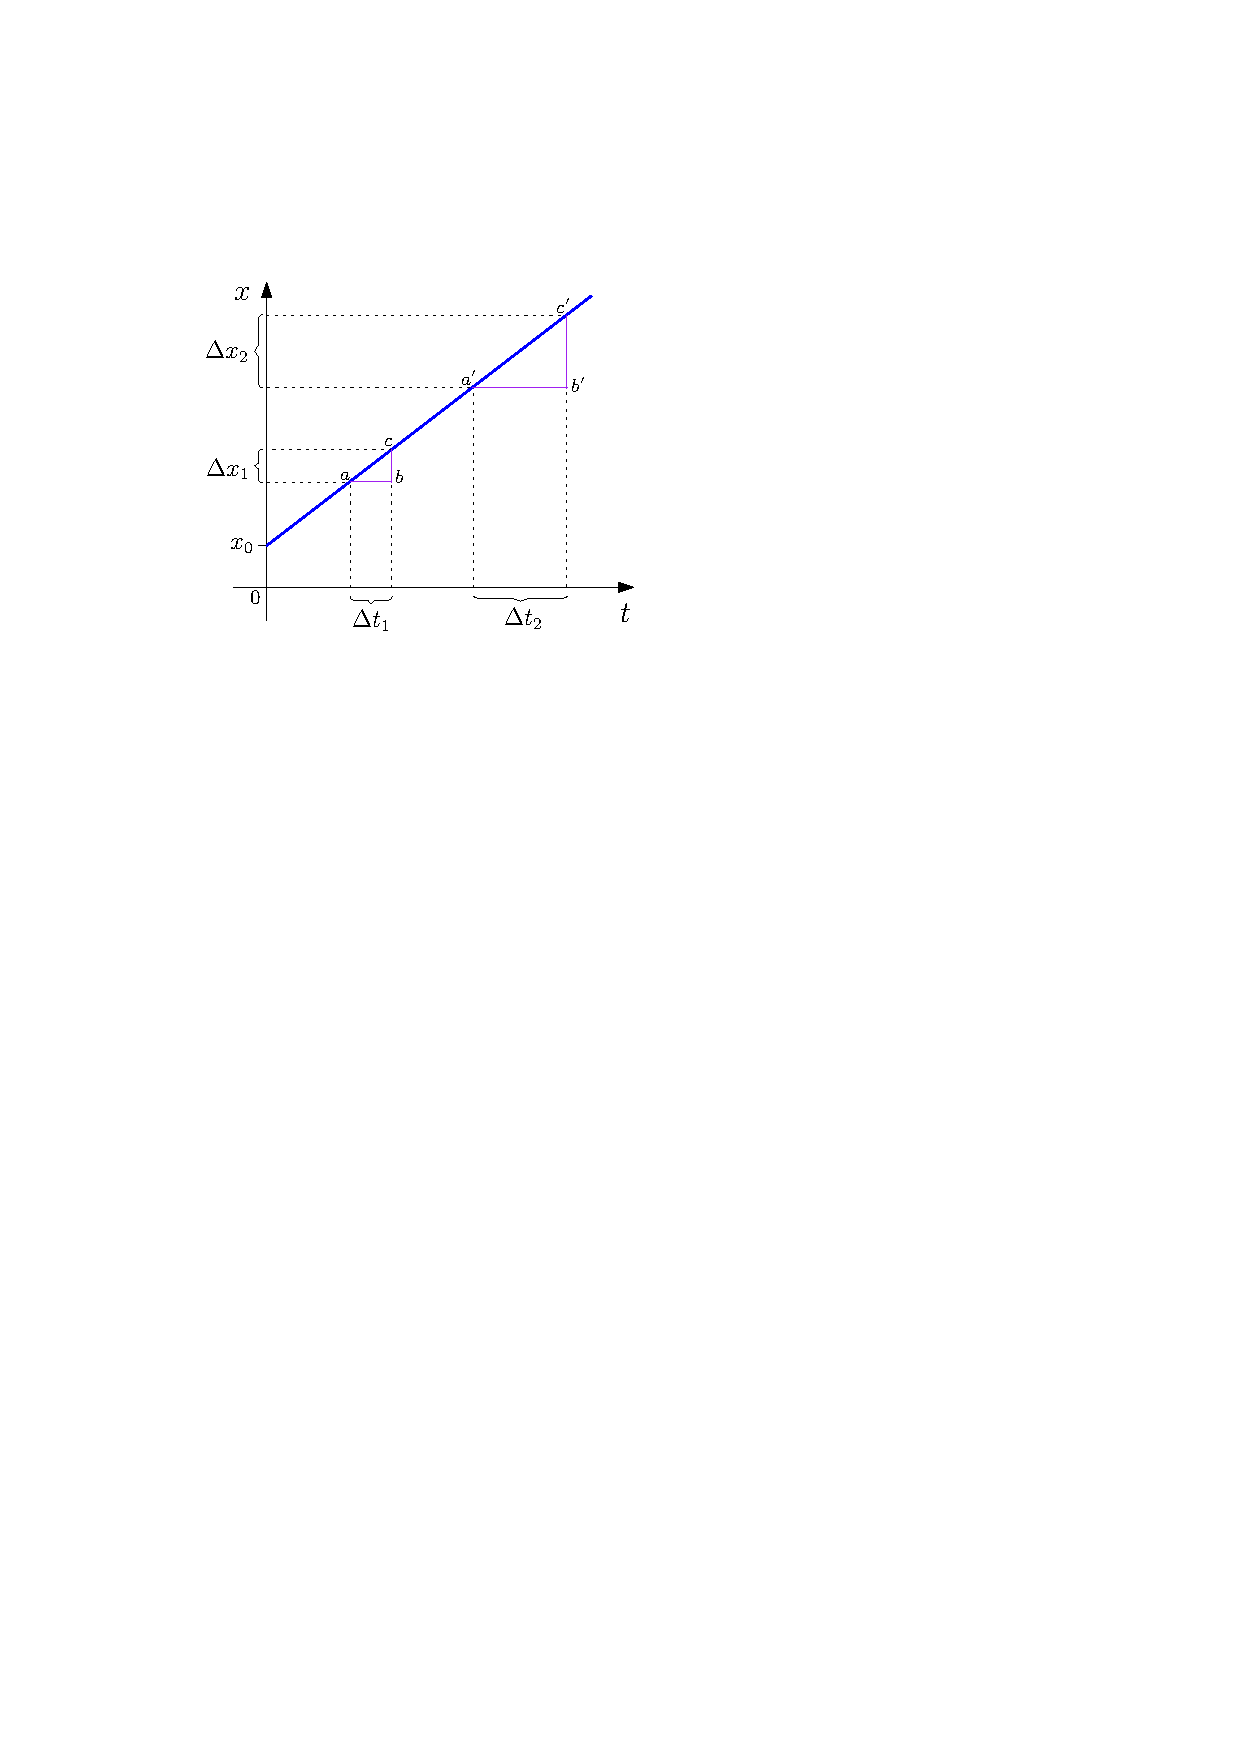
\includegraphics[scale=1]{img/MRU_intervalos.pdf}
  \end{center}
  ¿Qué tienen en común estos dos triángulos rectángulos? Dado que la rapidez es constante, podemos escribir
  $$v=\frac{\Delta x_1}{\Delta t_1}=\frac{\Delta x_2}{\Delta t_2}$$
  Es decir si dividimos {\it ``lo que varían las ordenadas''} por {\it ``lo que varían las absisas''} el cociente siempre es el mismo. Este cociente, constante para una recta, se llama {\bf pendiente}. Ahora podemos decir que, {\em en la gráfica $x=x(t)$ del MRU, la pendiente de la recta es la velocidad}.
\end{mybox}

\begin{comprension}
  \noindent
  {\bf Primero}  Analiza las siguientes gráficas:
  \begin{center}
    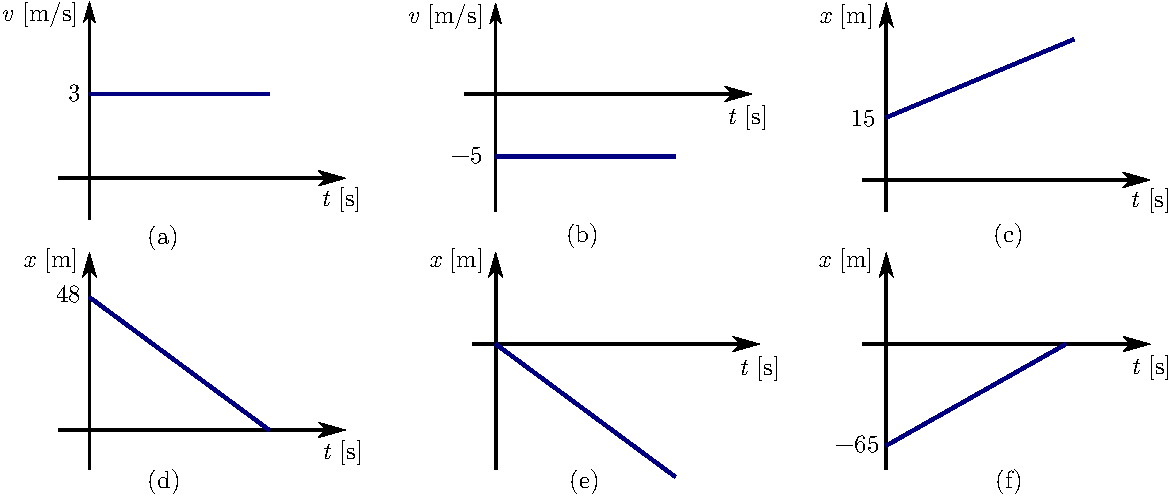
\includegraphics[width=0.9\textwidth]{img/analisisMRU.pdf}
  \end{center}

 \noindent
  {\bf Segundo} ¿Pueden la gráfica (b) y la (c) pertenecer a un mismo movimiento? Explica.
\end{comprension}
